%-----------------------------------------------------------------------------%
\chapter{\babEmpat}
\label{bab:4}

Bab ini menjelaskan detail arsitektur dan implementasinya. Perbedaan dari performa aplikasi ini memberikan kesempatan untuk melakukan optimisasi desain sistem terdistribusi ke depannya. Detail parameter dan cara melakukan tolok ukur performa terhadap variasi aplikasi PeerToCP juga akan dipaparkan lebih lanjut dalam bab ini pada subbab~\ref{sec:desain_evaluasi} tentang desain evaluasi. Bab ini juga akan memberikan penjelasan singkat serta alasan pemilihan beberapa teknologi, termasuk \textit{library} dan \textit{modul} yang digunakan dalam implementasi aplikasi PeerToCP. Sebagai konteks, bagian awal dari bab ini menjelaskan mengenai teknologi yang digunakan untuk implementasi, diikuti dengan desain sistem serta detail sudut pandang pengguna terhadap \textit{usecase} aplikasi.

\section{\textit{Library} dan \textit{Framework} Terkait}

Terdapat beberapa aplikasi dan \textit{library} yang terkait dalam pengembangan sistem aplikasi PeerToCP yang dibahas dalam penelitian ini. Berbagai \textit{framework}, \textit{library}, dan sistem modul ini merupakan hasil penelitian oleh para pengembang sebelumnya. Pemilihan penggunaan untuk setiap teknologi ini dipertimbangkan dengan alasan tertentu, salah satunya adalah Electron, yang menjadi basis pengembangan aplikasi \textit{desktop}.

Electron merupakan salah satu \textit{framework} aplikasi \textit{desktop} yang melibatkan HTML, CSS, dan JavaScript. Bagian belakang atau \textit{backend} dari Electron berjalan dengan lingkungan \textit{runtime} Node.js~\citep{kredpattanakul2018transforming, miglanielectron}. Node.js merupakan bahasa yang menggunakan \textit{syntax} yang serupa dengan Javascript dan dapat dikompilasi melalui kompilator yang disebut V8 engine~\citep{tilkov2010node}. Bagian tampilan atau \textit{frontend} dari Electron memanfaatkan aplikasi \textit{Chromium} yang dapat mengolah bahasa \textit{markup} web, seperti HTML (\textit{HyperText Markup Language}), CSS (\textit{Cascading Style Sheets}), serta JavaScript.

Salah satu keuntungan menggunakan Electron adalah aplikasinya yang bersifat \textit{cross-platform} atau dapat berjalan di beragam sistem operasi, seperti Windows, GNU/Linux, atau MacOS. Keuntungan lainnya ialah karena bersifat aplikasi desktop, Electron dapat mengakses berbagai macam fungsi antar muka sistem operasi, seperti memanggil subproses pada sistem dan menulis berkas. Karena \textit{frontend}-nya yang menggunakan bahasa web pula, aplikasi yang dibuat dengan Electron cenderung lebih mudah untuk dipindahkan dan diadaptasi dengan fungsi terbatas pada web. Selain \textit{Electron}, masih terdapat beberapa alternatif \textit{desktop-based framework} lain seperti Qt yang berbasis C++ dan Tauri yang berbasis Rust. Pemilihan Electron dipilih karena beberapa \textit{library} \textit{operational transformation}, \textit{CRDT}, \textit{WebSocket}, dan \textit{WebRTC} yang umum digunakan sudah tersedia implementasinya dalam JavaScript dan dapat digunakan melalui Node.js.

Untuk memenuhi kebutuhan komponen editor kode sebagai media interaksi pengguna dengan sistem pada \textit{frontend}, digunakan \textit{Codemirror}. Codemirror merupakan komponen \textit{frontend} editor kode yang dapat diolah oleh peramban web. Codemirror menyediakan banyak ekstensi, aksesibilitas tinggi, serta dukungan untuk berbagai macam bahasa pemrograman. Codemirror berguna untuk menampilkan editor kode dan memiliki ekstensi yang menghubungkannya dengan Yjs, sebuah library CRDT dan sudah diuji oleh pengembang Codemirror.

Yjs sendiri merupakan sebuah \textit{framework library} yang mengimplementasi CRDT yang disebut dengan YATA (\textit{Yet Another Transformation Approach})~\citep{Nicolaescu2016yjs}. Yjs terdiri dari beberapa bagian, yaitu YDocs yang merupakan bagian utama implementasi berbagai struktur data untuk CRDT. Dalam penelitian ini, digunakan tiga struktur data CRDT yang abstraksinya berbeda. YText merupakan variasi CRDT untuk operasi-operasi pada \textit{text editor}, serta YMap dan YArray yang dikombinasikan untuk menyimpan \textit{shell} dan riwayatnya. Yjs sendiri merupakan \textit{library} yang tidak terpaku pada sebuah arsitektur. Terdapat dua \textit{provider} jaringan yang dapat berintegrasi dengan YDocs, yaitu YWebRTC dan YWebSocket. Kedua provider ini masing-masing mengintegrasikannya dengan jaringan \textit{full-mesh peer-to-peer} dan \textit{client-server} secara berturut-turut. Yjs memiliki banyak pengembang aktif dari komunitas dan hingga kini masih di-\textit{maintain} dan dikembangkan, sehingga \textit{library} ini dipilih untuk penelitian ini.

Untuk variasi \textit{operational transformation} dari PeerToCP, penelitian ini memanfaatkan ekstensi \textit{collaborative editing} dari CodeMirror yaitu @codemirror/collab. Penyimpanan \textit{shell} diimplementasi tanpa \textit{operational transformation} karena dapat disimpan menggunakan \textit{array} yang bersifat \textit{grow-only}. Secara khusus, operasi penghapusan pada masukan \textit{shell} dapat dianggap sebagai menambahkan tiga karakter $\"\texttt{\b \b}\"$ atau ekuivalen dengan memindahkan ke cursor ke kiri, tanpa menghapus karakter. Sementara \textit{provider} jaringannya dikembangkan dalam penelitian ini menggunakan \textit{library} rpc-websockets yang dimodifikasi sehingga dapat dimanfaatkan untuk melakukan \textit{broadcast}, \textit{specific-messaging} ke klien tertentu, serta fungsionalitas pemanggilan RPC (\textit{Remote-Procedure Call}) berbentuk \textit{promise} secara \textit{asynchronous} dan \textit{non-blocking}.

Untuk memenuhi komponen penjalanan program yang dapat diakses oleh setiap klien dalam jaringan, dibutuhkan suatu \textit{library} untuk mengakses sistem operasi untuk melakukan kompilasi terhadap kode. Kompilasi merupakan proses mengonversi kode dari bahasa dengan level yang lebih tinggi dan dapat dimengerti oleh manusia menjadi kode biner yang dapat dimengerti oleh mesin~\citep{aho1985compilers}. Pada penelitian ini, selain editor kode yang bersifat kolaboratif, proses kompilasi kode tunggal juga hendaknya dapat dilakukan oleh salah satu pengguna. Proses kompilasi ini membutuhkan kompilator yang terpasang pada suatu sistem operasi. Pada Node.js, salah satu \textit{library} yang dapat digunakan untuk mengaksesnya ialah Node-pty.

Node-pty merupakan \textit{library} Node.js yang memberikan antarmuka untuk melakukan \textit{fork} proses dengan deskriptor berkas \textit{pseudoterminal}. Node-pty mengizinkan adanya aliran data untuk baca dan tulis dengan proses berjalan pada kernel. Node-pty berguna untuk menjalankan berkas hasil kompilasi yang bersifat CLI (\textit{Command Line Interface}) yang tidak memiliki tampilan grafik untuk pengguna. Node-pty dipilih karena banyak digunakan dan bersifat \textit{cross-platform} mendukung sistem operasi Windows, GNU/Linux, dan MacOS. Aplikasi ini juga membutuhkan bagian \textit{frontend} untuk menampilkannya, dan digunakan Xterm.js. \textit{Library} ini merupakan salah satu komponen yang menampilkan terminal melalui bahasa yang dapat diolah oleh web. Xterm.js memiliki antarmuka yang bisa menerima dan meneruskan data dari peramban (\textit{browser}) yang dapat dihubungkan dengan sebuah proses berjalan pada sistem. Xterm.js dikembangkan tanpa memerlukan dependensi, sehingga dipilih dalam pengembangan sistem ini.

\section{Desain Sistem}

Aplikasi PeerToCP didesain sebagai sebuah aplikasi \textit{desktop-based}, yang berarti dijalankan tidak melalui browser \textit{web}. Pilihan ini dikonsiderasi karena untuk mempermudah akses secara \textit{offline}, sehingga tidak dibutuhkan koneksi internet untuk mengakses aplikasi. Selain itu, fitur kompilasi pada suatu \textit{peer} memerlukan akses \textit{system-call} yang tidak disediakan pada API web-browser~\citep{v8, spidermonkey}. Hal ini ditetapkan agar \textit{script} yang dijalankan pada mesin browser tidak dapat menyerang komputer secara langsung. Berikut ialah \textit{diagram activity} yang menunjukkan garis besar penggunaan aplikasi.

\begin{figure}
    \centering
    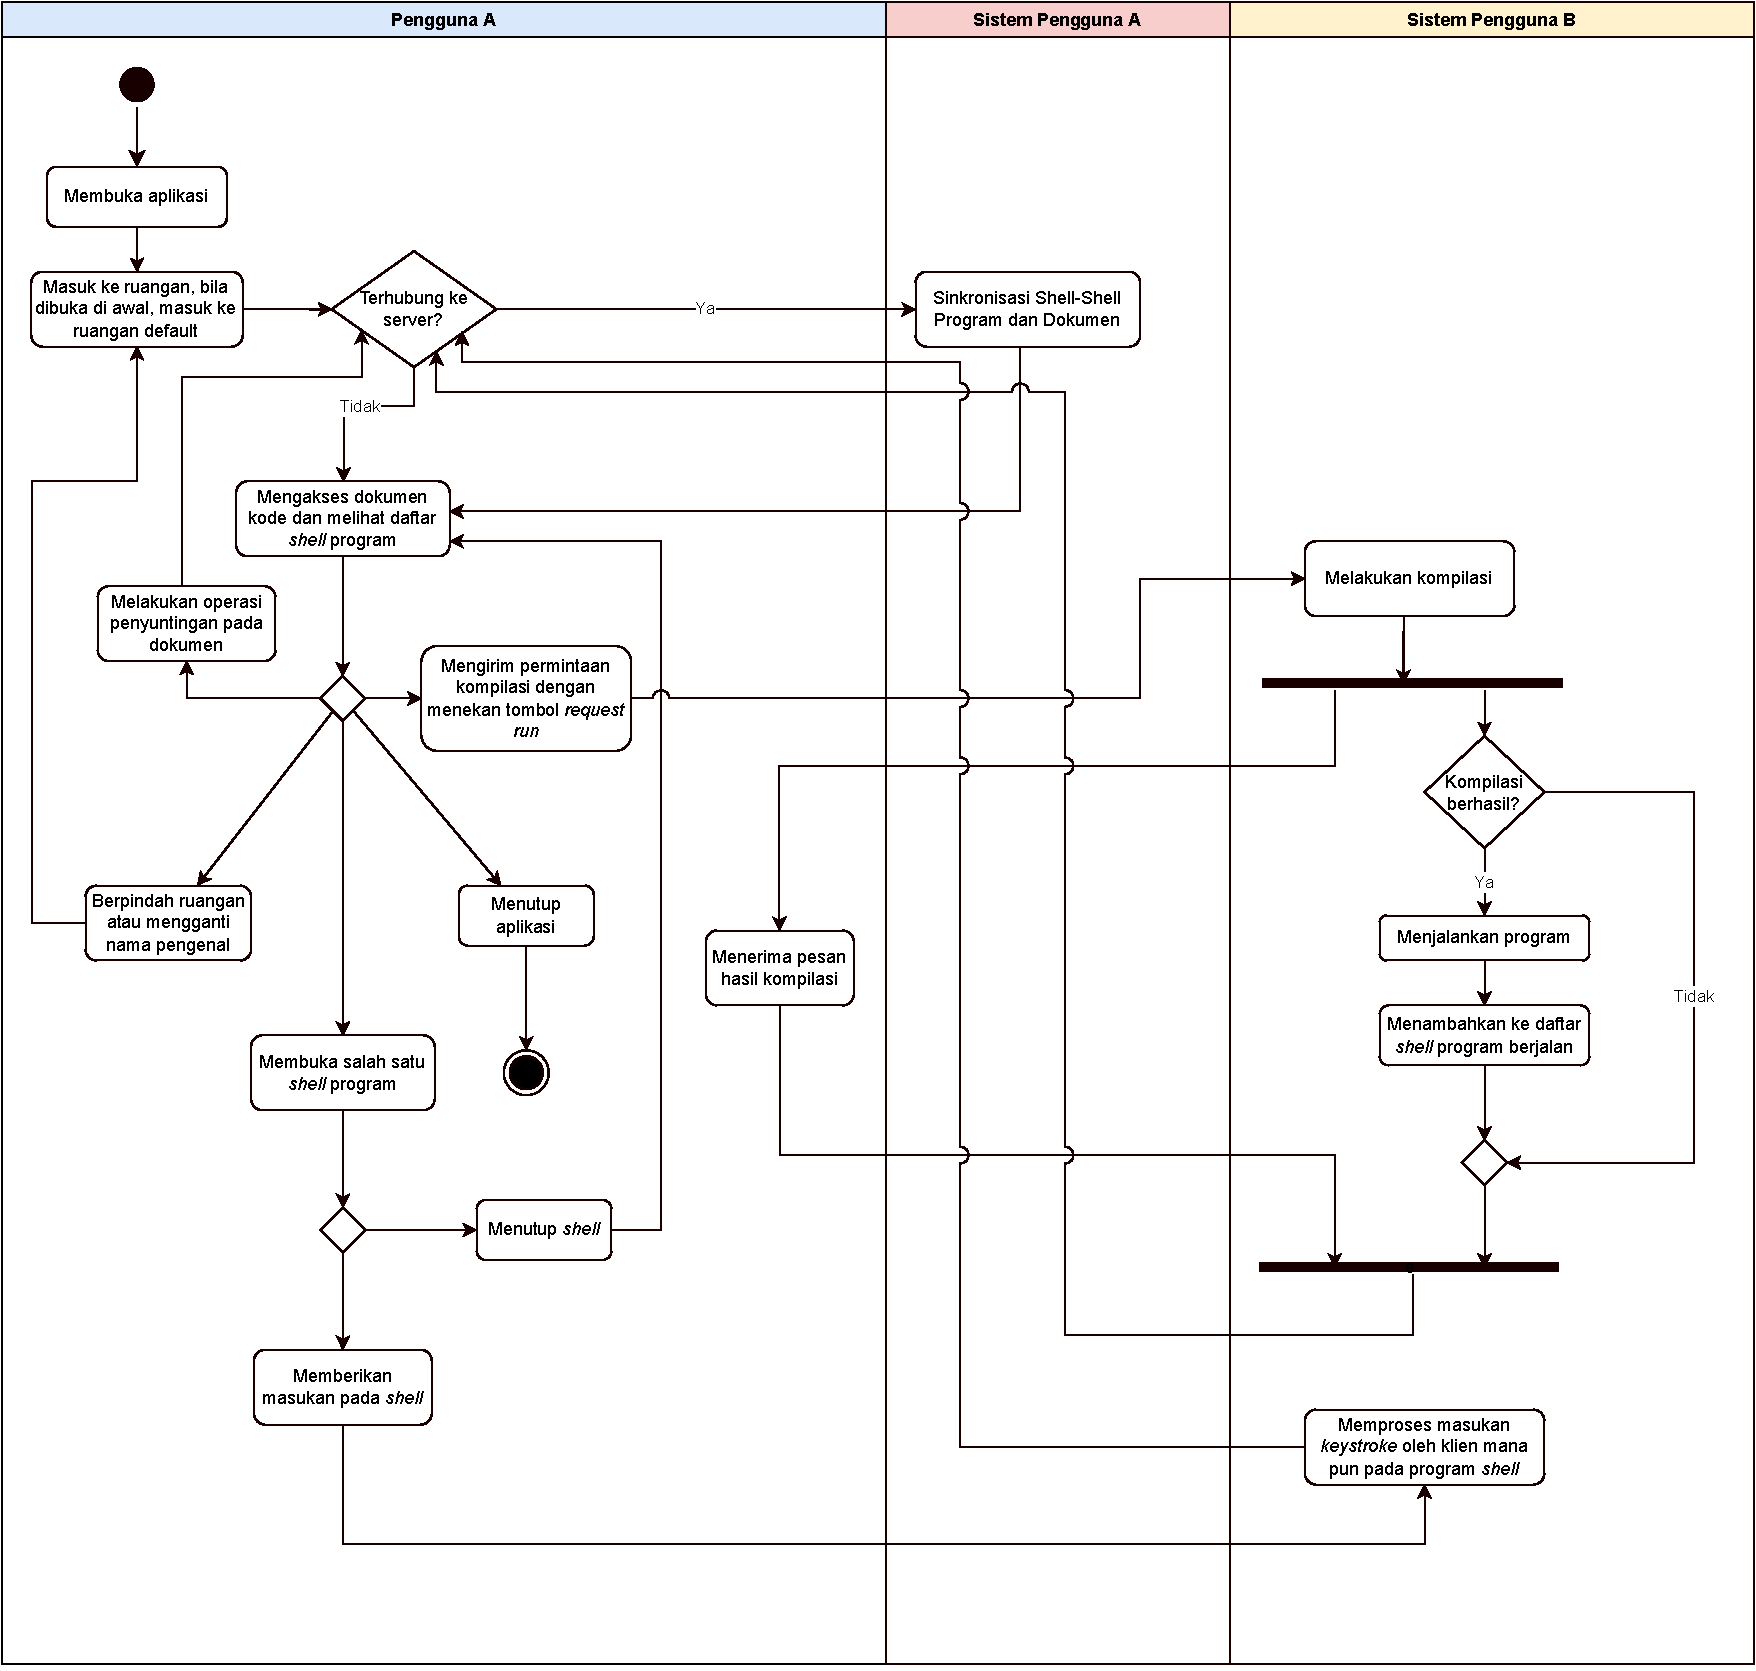
\includegraphics[scale=0.5]{assets/skripsi/Activity_Diagram}
    \caption{\textit{Activity Diagram} Alur Penggunaan Secara \textit{High Level}}
    \label{fig:activity}
\end{figure}

Saat pengguna membuka aplikasi, pengguna akan diarahkan untuk masuk ke ruangan awal secara \textit{default}. Pengguna dapat melakukan operasi-operasi penyuntingan pada dokumen dan sinkronisasi dilakukan secara terus-menerus dengan \textit{publish-subscribe design pattern} sehingga memberikan respons tanpa perlu mengecek atau \textit{polling} secara terus menerus saat terjadi \textit{update} yang terjadi antarklien. \textit{Request} atau permintaan kompilasi dapat diajukan kepada klien mana pun pada jaringan, termasuk permintaan untuk klien ini sendiri. Aplikasi PeerToCP akan mencoba mengirimkan pesan kepada klien yang ditentukan tanpa mengabari tanpa intervesi dari klien lain dalam jaringan. Apabila permintaan berhasil diterima, sistem pada klien yang diminta akan melakukan proses kompilasi dan memasukkan \textit{shell} program berjalan dengan \texttt{id} tertentu ke daftar \textit{shell} yang dapat diakses ke setiap klien dalam jaringan. Daftar \textit{shell} dan kontennya ini disimpan dalam bentuk \textit{object} pada \textit{JavaScript}.

Pada Gambar~\ref{fig:activity}, perilaku sinkronisasi \textit{shell-shell} program dan dokumen dilakukan tergantung dengan variasi implementasi dari program. Pada arsitektur \textit{client-server}, sistem aplikasi pengguna A akan berhubungan dan melakukan sinkronisasi dengan server. Sementara pada arsitektur \textit{peer-to-peer}, sistem aplikasi pengguna A akan berhubungan langsung dan melakukan sinkronisasi dengan \textit{peer} atau klien lain. Selain itu, permintaan dan transmisi pesan hasil kompilasi dilakukan melalui pengiriman pesan secara langsung pada arsitektur \textit{peer-to-peer}, namun harus melalui perantara server pada arsitektur \textit{client-server}. Detail implementasi dan arsitektur detail aplikasi akan dirincikan pada Bab~\ref{bab:4} Implementasi. Sistem yang telah dikembangkan kemudian akan dilakukan evaluasi secara objektif berdasarkan aspek-aspek tertentu yang menrepresentasikan performa dan skalabilitas aplikasi.

\section{Arsitektur Peer-To-Peer}

\begin{figure}
    \centering
    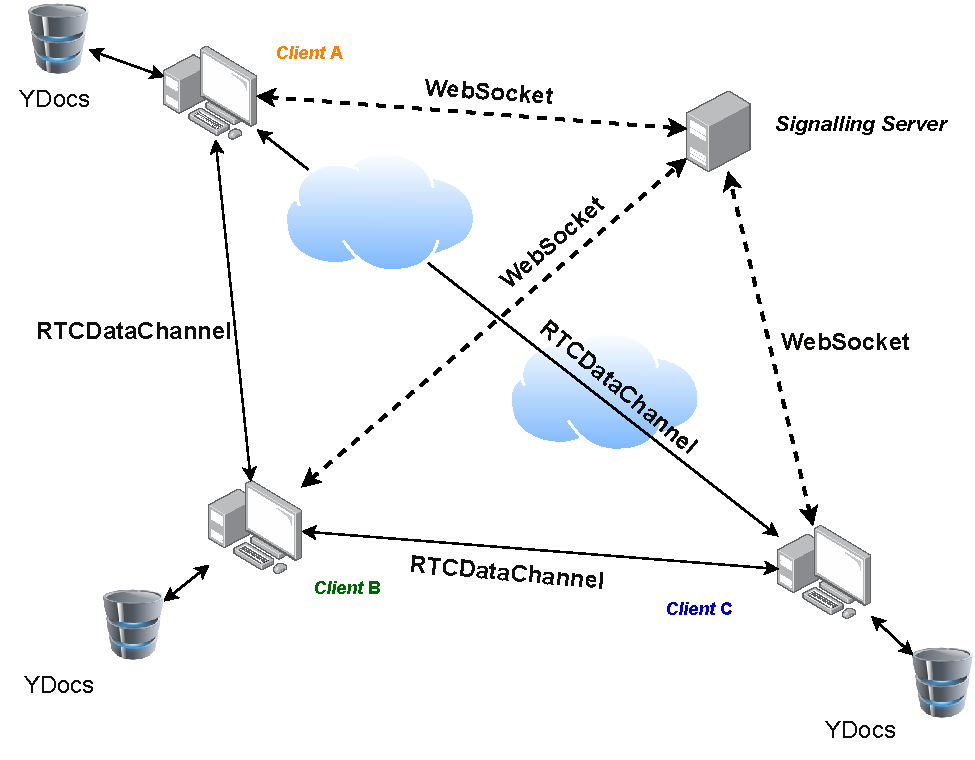
\includegraphics[scale=0.6]{assets/skripsi/Arsitektur_WebRTC_CRDT}
    \caption{Arsitektur WebRTC-CRDT}
\end{figure}

\section{Arsitektur Client-Server}

\begin{figure}
    \centering
    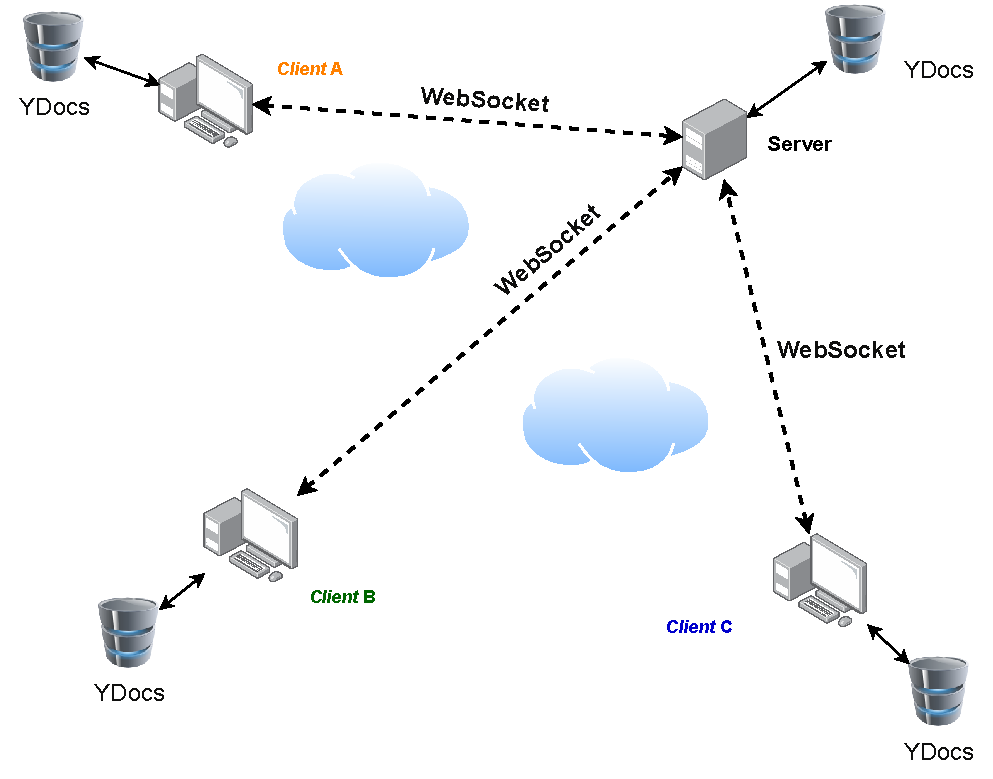
\includegraphics[scale=0.42]{assets/skripsi/Arsitektur_WebSocket_CRDT}
    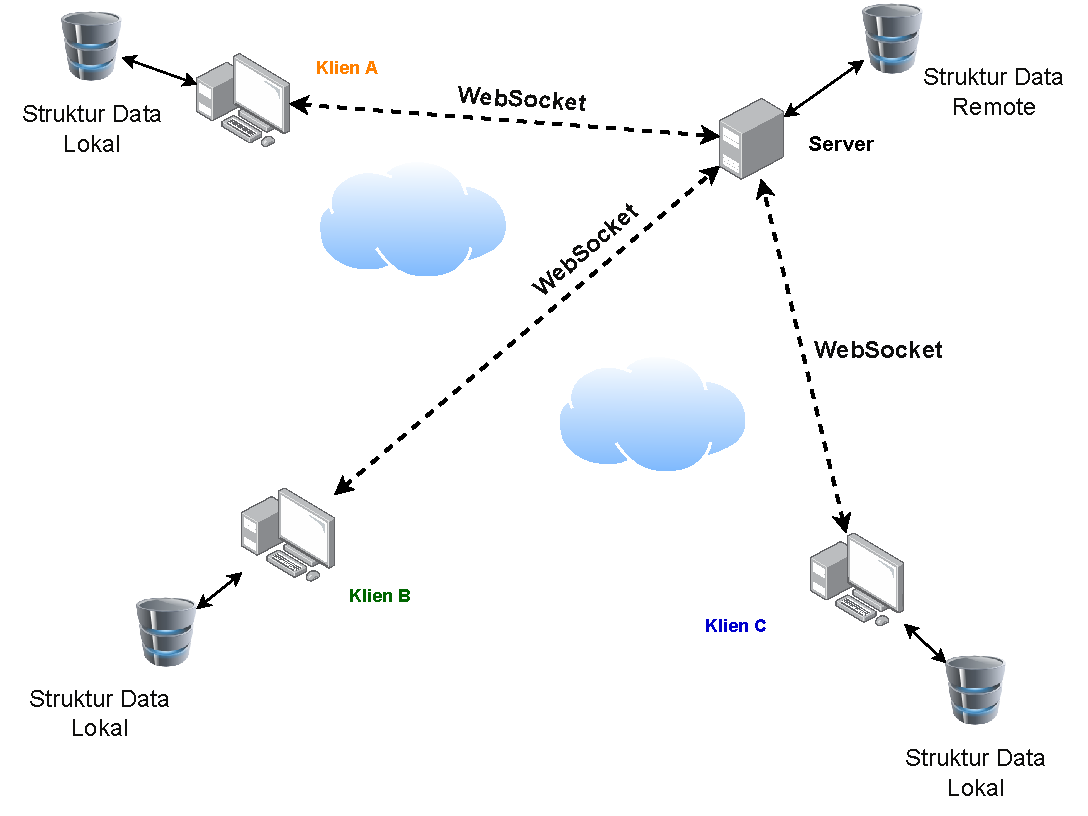
\includegraphics[scale=0.42]{assets/skripsi/Arsitektur_WebSocket_OT}
    \caption{Arsitektur WebSocket-CRDT dan WebSocket-OT Secara Berurutan}
\end{figure}


\section{Desain Evaluasi}
\label{sec:desain_evaluasi}